\section{System Prototype}
\label{sec:design}

Shown in Figure\ref{fig:proto} is a diagram illustrating our initial prototype of CommunityGuard, where we focus on running an intrusion prevention system (Snort) as the example network function (which can do both monitoring and protection, but our architecture is not solely tied to Snort).  

%\begin{figure}
    %\centering
    %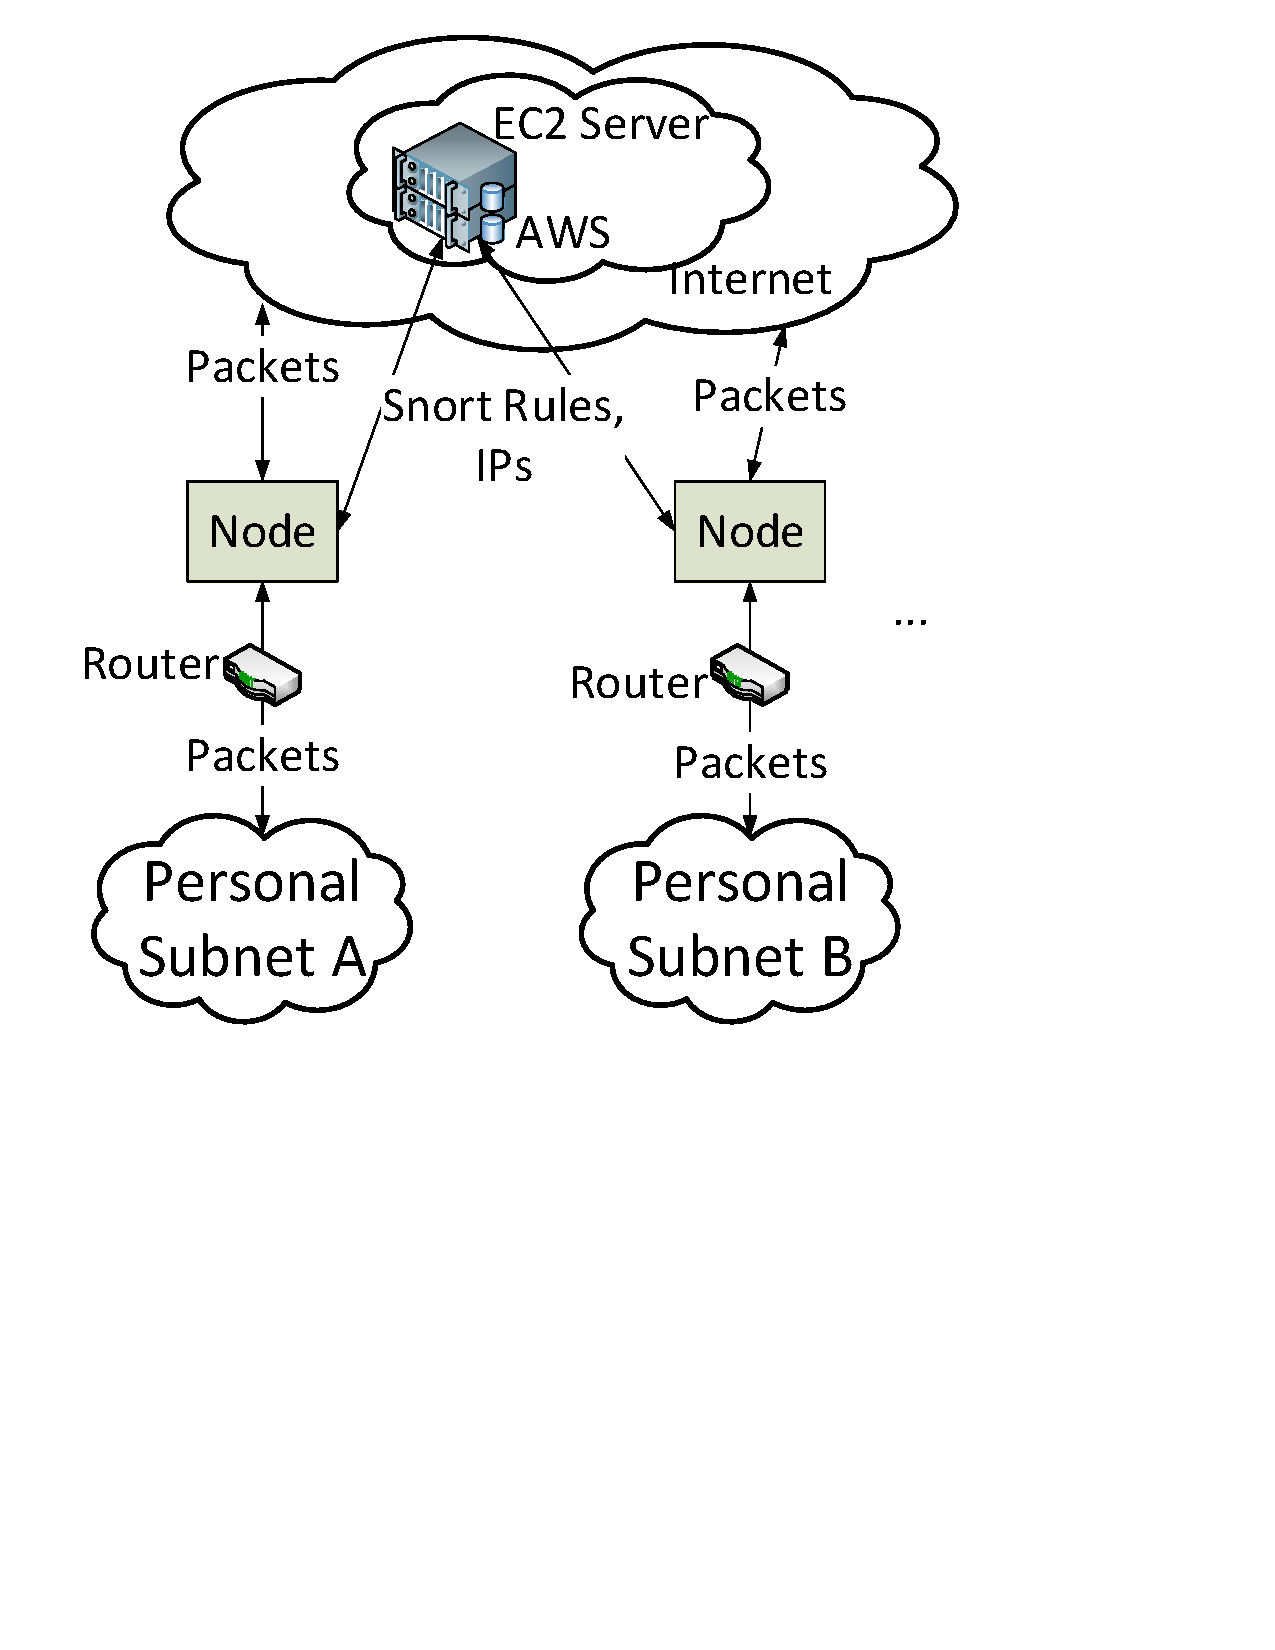
\includegraphics[height=4.4cm]{figs/macroarch.pdf}
    %\caption{Community Guard macro-level prototype overview.}
    %\label{fig:macro}
%\end{figure}


\begin{figure}
    \centering
    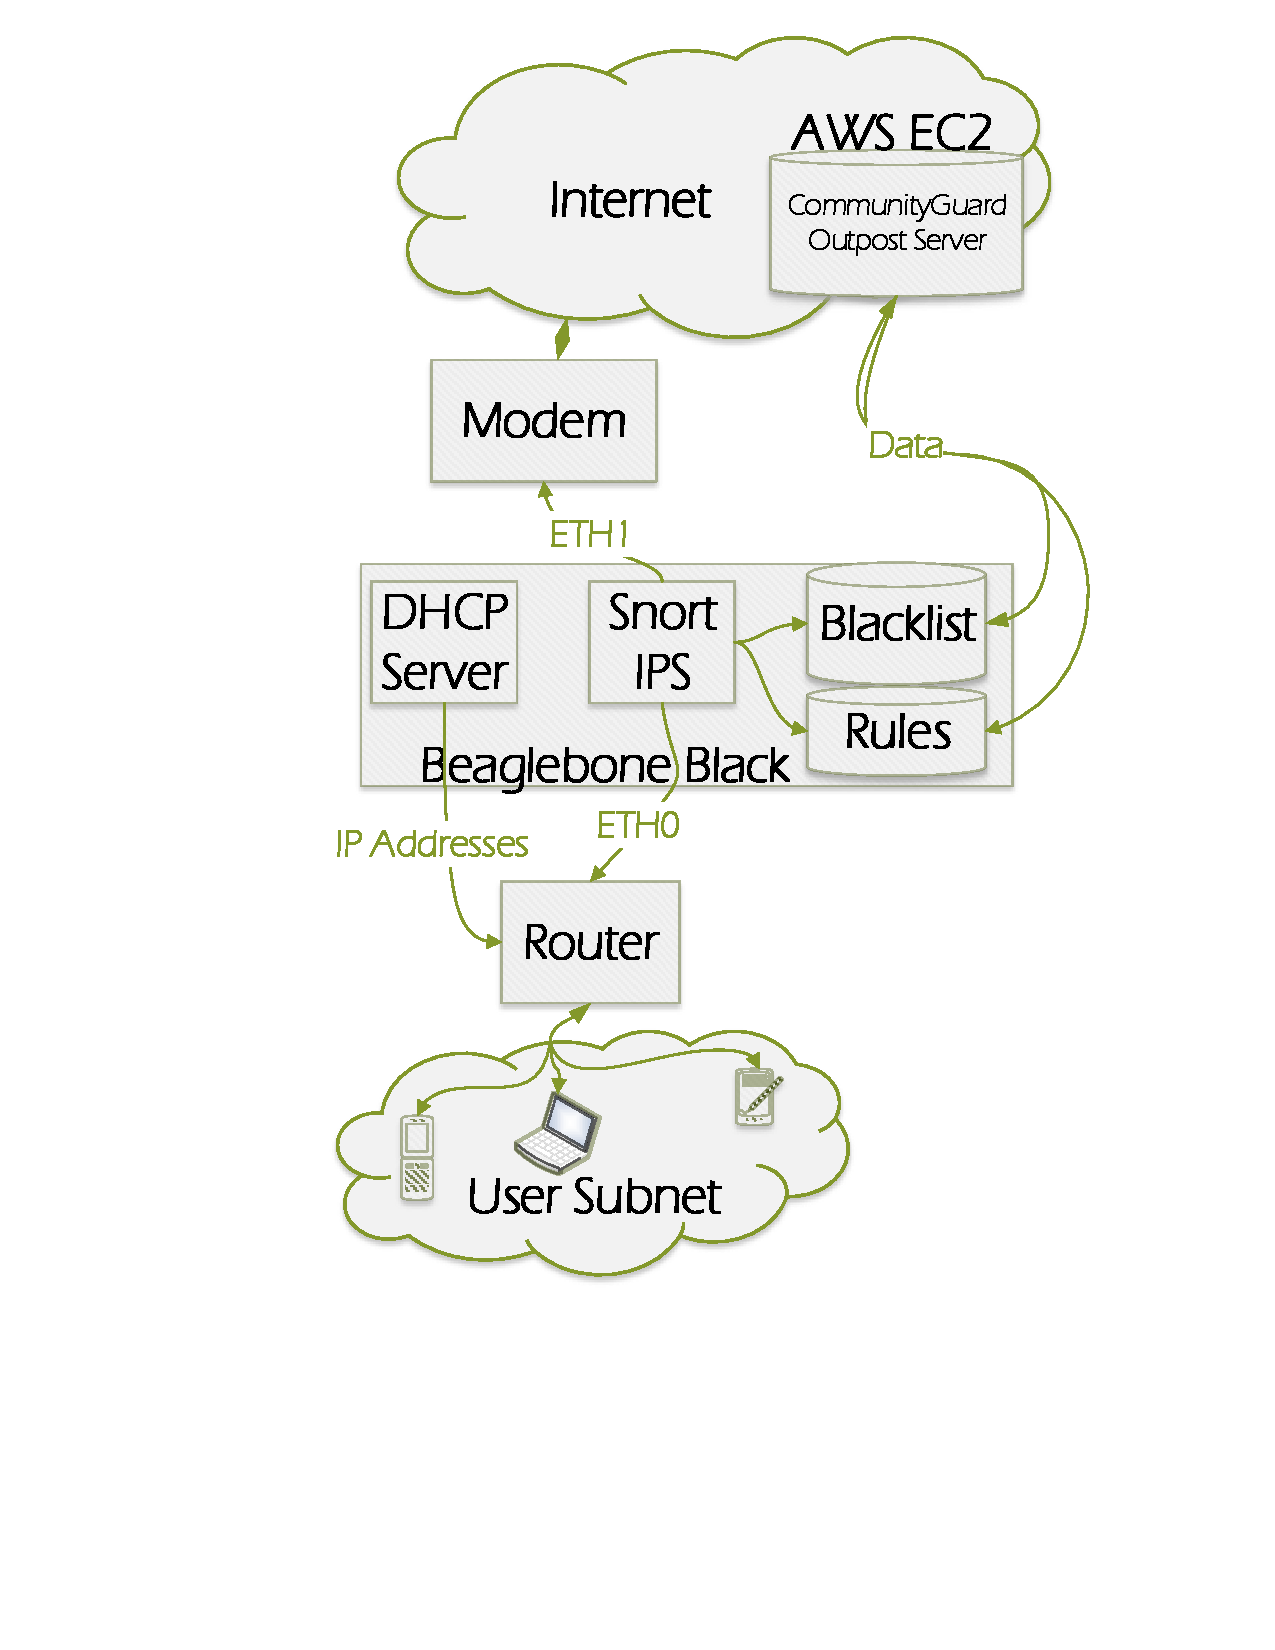
\includegraphics[width=0.75\columnwidth]{figs/microarch.pdf}
    \caption{Prototype Overview.}
    \label{fig:proto}
\end{figure}

The keystone of the proposed architecture is the Guardian Node which must be placed in a position where it can view the entire network traffic flowing into and out of a user's network, and block all suspicious traffic. The addition of the device must be as non-intrusive as possible, requiring no modification in Modem or Router configuration.
Based on these factors, we chose to place the Guardian Node between a Modem and Router. For networks using a Modem and a Router on the same device, we foresee that a production scale implementation would place the Guardian Node within the same box as the Modem and the Router, therefore maintaining the same architecture as shown in Figure~\ref{fig:arch}. Such Guardian Nodes placed at the entry point of home networks can create a solid net of protection that can communicate threats as soon as they emerge. It must be noted that the capability of CommunityGuard in deterring threats (and especially its ability to stop DDoS attacks) is proportional to the amount of subnets that use it -- ideally there would be a Guardian Node within every household and business subnet.

The code that we wrote in implementing and evaluating CommunityGuard is available on Bitbucket at \\ https://bitbucket.org/ChaseEStewart/advnetsysfinal/ \cite{us}.

\subsection{Guardian Node}
\label{sec:design:guardian}

\subsubsection{Guardian Node Design}
The BeagleBone Black, a reasonably powerful embedded device, was chosen to prototype Guardian Node since it satisfied the minimum requirements to implement the envisioned end product. The on-board 10/100 Mbps Ethernet port provided one network interface, while another interface was added using an USB to 10/100 Mbps Ethernet adapter. This prototype is deemed sufficient to display the core mechanics of the Guardian Node. 

\subsubsection{Software Design}
\label{sec:design:software}

The software design of a Guardian Node is depicted in Figure~\ref{fig:proto}. The device has a DHCP server configured so that a Router can be added behind it. It passes all traffic from one network interface to the other. The Guardian Node runs Snort \cite{Roesch:1999:SLI:1039834.1039864}, a powerful Intrusion Detection/Prevent tool, to monitor traffic at both interfaces. A set of Snort rules are configured to block any suspicious traffic that satisfies any of the rules. Snort can perform protocol analysis, content searching/matching, and can be used to detect a variety of attacks and probes, such as buffer overflow, stealth port scans, CGI attacks, SMB probes, OS fingerprinting attempts, and many more. It also provides a black-list and white-list functionality that can be used to conditionally block and unblock malicious IP addresses. Snort was chosen as the IPS due to its large amount of documentation, open source software and up-to-date rule-lists, and its high regard in security communities.

Communication of malware alerts is a key aspect of CommunityGuard. This communication is done on a periodic basis by a set of three cron jobs running on the Guardian Node. These cron jobs do the following:

\begin{itemize}
    \item Keep Snort's general rules up-to-date by pulling rules and IPs from rule repositories.
    \item Push this particular guardian node's suspicious traffic to the Community Outpost and also to pull new rules and blocked IPs from the Community Outpost.
    \item Check for DDoS server beacons and generate new anti-DDoS rules if necessary.
\end{itemize}

The first cron job runs periodically and reads a log created by Snort that contains IP address of sources that have sent bad traffic. It then parses the source IP addresses present in the log, and updates the same to the database on the Community Outpost (described in the following section).

\begin{figure}
    \centering
    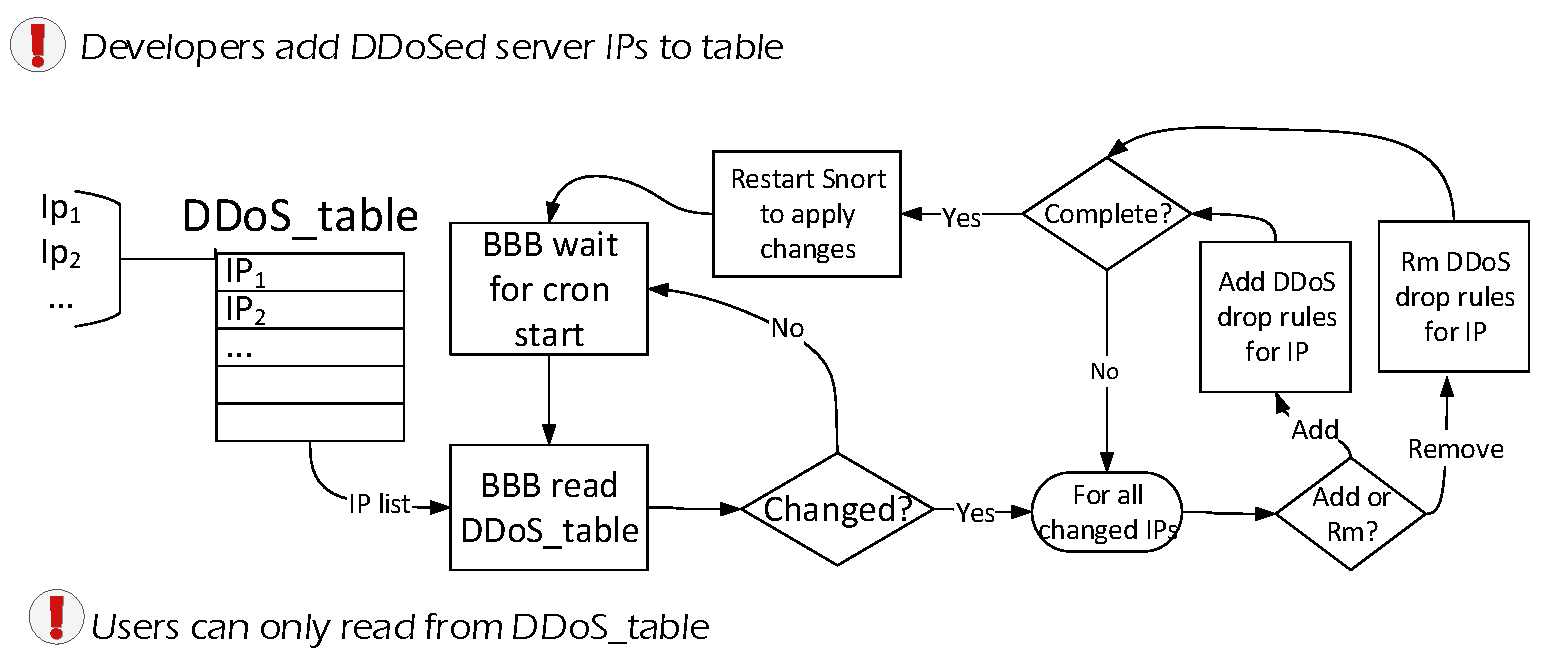
\includegraphics[width=0.95\columnwidth]{figs/ddosserv.pdf}
    \caption{Outbound DDoS prevention Algorithm}
    \label{fig:ddostable}
\end{figure}



A second cron job runs periodically to fetch information from a DDoS watch list available on the Community Outpost described below as part of the Outgoing DDoS prevention mechanism (server-side is described in Section \ref{sec:design:serverddos}). If the database provides new IP addresses (for which rules do not exist on the Guardian Node yet) that are currently being DDoSed, the cron job creates and adds Snort rules to drop all such outgoing DDoS traffic, thus clipping off the attack at the compromised source itself. 
This algorithm is depicted in Figure ~\ref{fig:ddostable}; Such a mechanism, when repeated over all Guardian Nodes, can prevent a DDoS attack from the source.

Finally, the third cron job runs once every day at some random time and fetches the latest bad IP list from the Community Outpost and adds it to the Snort IP Blacklist. It also fetches Snort rules from Emerging Threats ~\cite{emerging} to defend against new and emerging attack patterns. These three cron jobs, combined with Snort running on all Guardian Nodes, together establish a system of protection that learns, communicates, and has the capacity to prevent most malware attacks.

\subsection{Community Outpost}
\label{sec:design:server}

% TODO I know I need to crop this
\begin{figure}
    \centering
    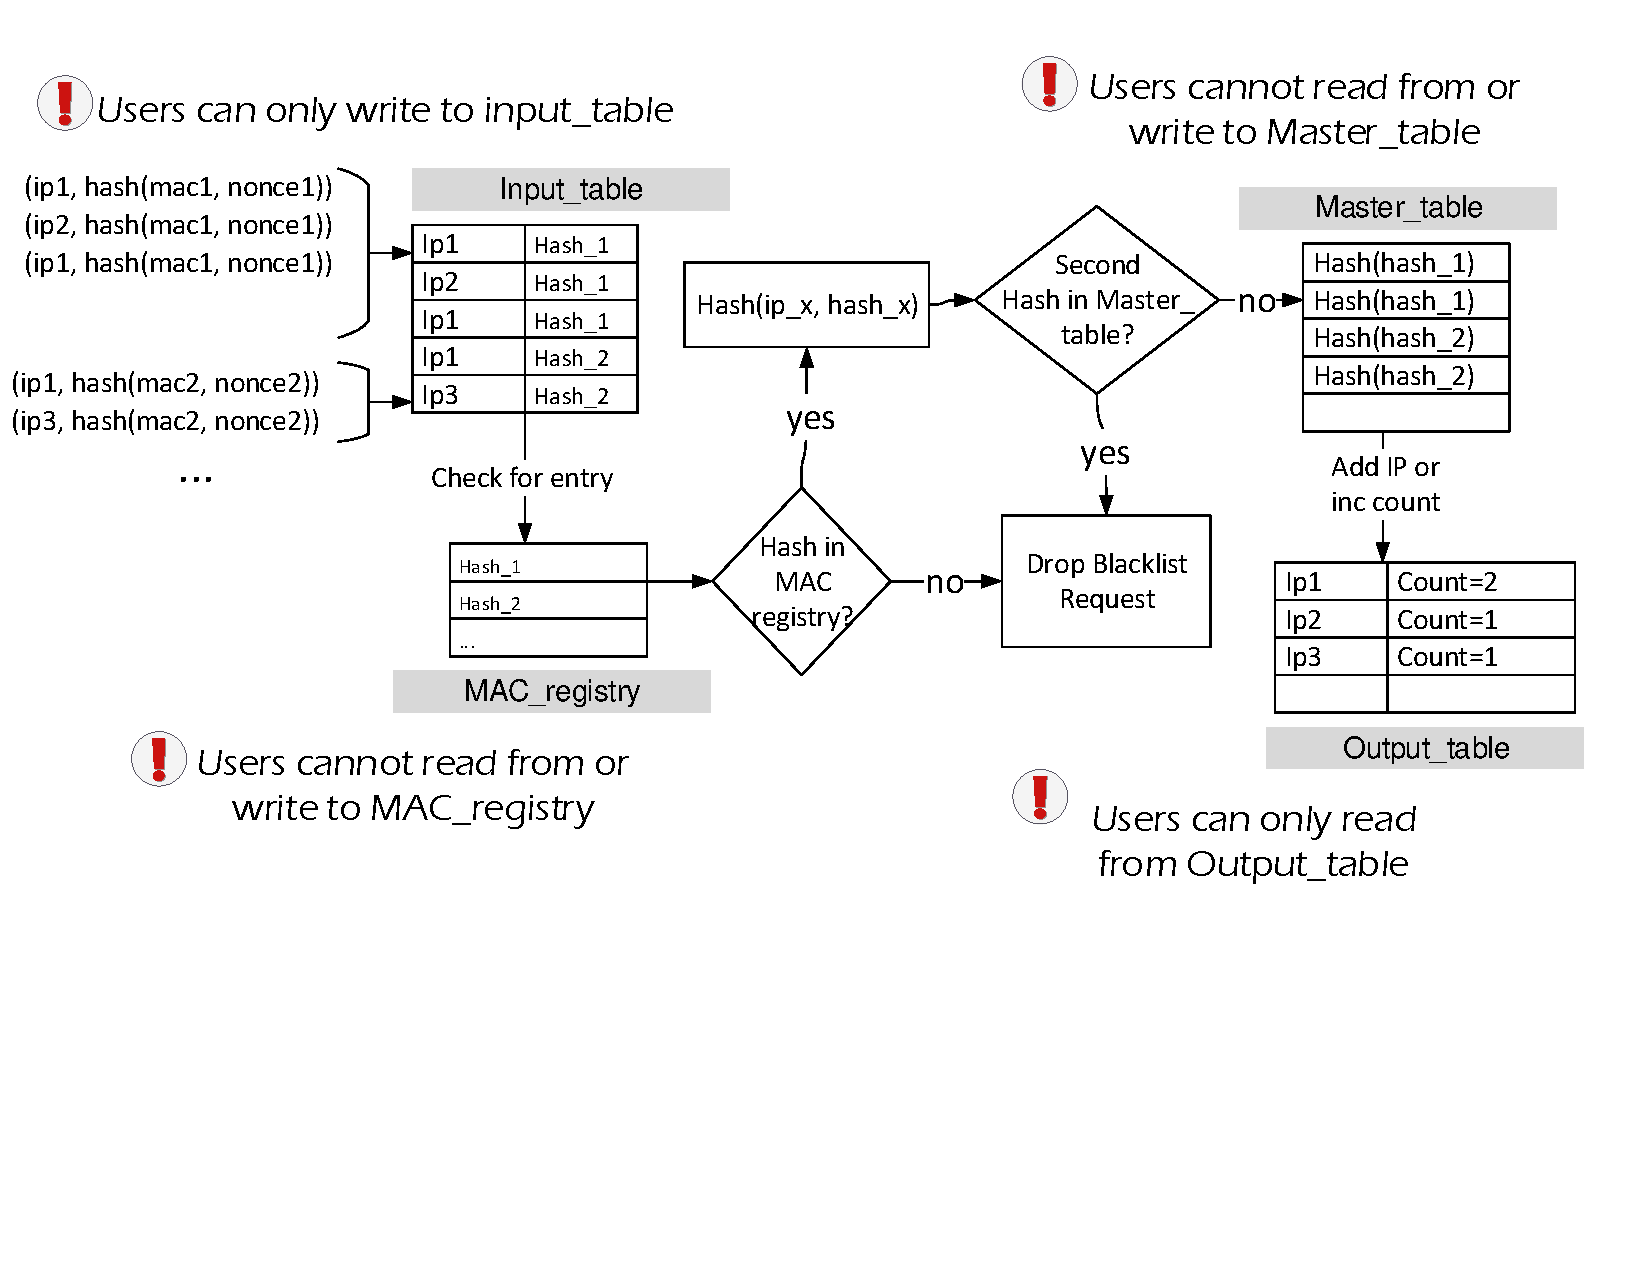
\includegraphics[width=0.95\linewidth]{figs/blacklist.pdf}
    \caption{Community Outpost push and pull.}
    \label{fig:blacklistserver}
\end{figure}

The Community Outpost is the source of intelligence for the Guardian Nodes that it services. This server runs a database and a couple of cron job timed events to process the information within its database. This server uses its database tables to aggregate threats presented by all collected guardian nodes, process them to determine valid threats, and then present them for individual guardian nodes to read and process. As this server is an obvious target for one who would wish to halt the CommunityGuard service, it is foreseen that the server will be elastically-scaling and secure in a production level implementation. 

\subsubsection{Attack Models}
\label{sec:design:attacks}
We assume that a user will not attempt to attack or compromise the availability or function own Guardian Node since our system aims to protect users who are unaware that their devices have been compromised. Furthermore, the Guardian Node itself can be fortified from external attacks through a hardened OS image and security best practices. This leaves a malicious user two possible vectors of attack for causing harm to a particular user- either attempting to get harmful traffic through the Guardian Node, or else reverse-engineering the Guardian Node to attack the Community Outpost itself. 
We designed the functionality of the Community Outpost while keeping the following attack models in mind:

A malicious user may attempt to:
\begin{enumerate}
\item add useful IPs to the blacklist to block them for users
\item remove blacklisted IPs from the blacklist
\item read user data from the list
\end{enumerate}

\subsubsection{Server Blacklist architecture}
\label{sec:design:blacklist}
When any guardian node is created, a SHA256 hash of the node's MAC address and a random nonce stored on the Guardian Node's memory is entered into the mac_addr_registry table, as shown in Figure ~\ref{fig:blacklistserver}. This hash value will serve as a key for writes, to ensure that writes can only be initiated from a valid Guardian Node.

The Guardian Node is only allowed write permission to the IPv4_input table and read permission from the IPv4_output table and DDoS_output table. This policy prevents attack models 1, 2, and 3 and ensures that even if a malicious user were to reverse-engineer the device to discover a means to contact the Community Outpost directly, the amount of damage they could cause is minor. When a Guardian Node is scheduled to push suspicious traffic to the Community Outpost, it is allowed to write only into the IPv4_input table. It will write the following pair to the input table: \[\{ip_{suspicious}, SHA256(int(MAC addr), nonce)\}\] 

The Community Outpost will process the input table to recalculate new threats at a certain frequency, and then drop the current input table. For each entry in the input table, the server first checks the SHA256 passed by the Guardian Node to ensure that this key is already within the mac_addr_registry. The entries that do not have a valid SHA256 hash are dropped, leaving only the valid requests. For all valid requests, a second SHA256 hash is computed, this time a hash of both the previous SHA256 result and now also the IP address declared as suspicious \[SHA256(\{ip_{suspicious}, SHA256(int(MAC addr), nonce)\}) \]. The Community Outpost checks whether this hash is already in the IPv4_master_list server, which is a list of the SHA256, IP combinations that have previously been entered- if this is a new suspicious IP, or it is a known suspicious IP being reported by a new and valid Guardian Node, it will be pushed to the IPv4_output table. This second hash function ensures that a given Community Outpost instance receives only one vote towards a given IP address, as a means to prevent against attack model 1. 

If this IP is a new entry, it will be entered into the table with a count of 1; if it already exists within the table, its count will be incremented. Once the count tallied against the IP reaches a sufficiently high number proportional to the number of reported threats, the IP will be pushed as output to requesting Guardian Nodes, and blocked automatically by all Guardian Nodes. Relying on a count before pushing a suspicious IP also helps prevent attack model 1 from occurring. 

\subsubsection{Server Outgoing DDoS prevention}
\label{sec:design:serverddos}

As mentioned above in Section ~\ref{sec:design:software}, the Community Outpost also provides a method to prevent outgoing DDoS traffic from a Guardian Node's subnet out to a DDoS target. This system is much more simple than the blacklist method described above: in this case, the DDoS victim list will be edited by CommunityGuard administrators, and only reading will be allowed for all Guardian Nodes. CommunityGuard administrators will confirm the existence of a DDoS attack through an alternate channel, possibly a third party DDoS \cite{DDoSPreventionTools} working with CommunityGuard administrators, and then add the relevant IPs or CIDR ranges to the IPv4_ddos table. Guardian Nodes will use the cron described above to add and remove rules to prevent outgoing DDoS attacks.